\medskip

\textbf{Les questions 1, 2, 3 et 4 sont indépendantes les unes des autres.}

\medskip

\textbf{Question 1}

\medskip

On considère la fonction $f$ définie sur $\mathbb{R}$ par :
\[f(x) = (8x + 1)\e^{-x}.\]

On admet que $f(x) \geqslant 0$ pour tout $x$ appartenant à $[0~;~2]$.

Dans le repère orthonormé \Oij{} ci-dessous, $C_f$ désigne la courbe représentative de $f$.

\begin{center}
\begin{tikzpicture}[x=3cm,y=3cm,xscale=0.7,yscale=0.7,>=Latex]
\fill[pattern={Lines[angle=45,distance=7pt,line width=0.45pt]}, pattern color=orange!80!black]
  (0,0) -- plot[domain=0:2,samples=100] (\x,{(8*\x+1)*exp(-\x)}) -- (2,0) -- cycle;
\foreach \x in {1,2,3,4,5}
  \draw[gray!65, line width=0.5pt] (\x,0) -- (\x,3.75);
\foreach \y in {1,2,3}
  \draw[gray!65, line width=0.5pt] (-0.85,\y) -- (5.5,\y);
\draw[orange!80!black, line width=0.8pt]
  (0,0) -- plot[domain=0:2,samples=100] (\x,{(8*\x+1)*exp(-\x)}) -- (2,0);
\draw[blue, line width=1.5pt, domain=-0.18:5.45, samples=200, smooth]
  plot (\x,{(8*\x+1)*exp(-\x)});
\draw[->, line width=1pt] (-0.85,0) -- (5.5,0);
\draw[->, line width=1pt] (0,-0.35) -- (0,3.75);
\foreach \x in {1,2,3,4,5}
  \node[below] at (\x,0) {\small \x};
\node[below left=-1pt] at (0,0) {\scriptsize 0};
\node at (0,0) {$\times$};
\foreach \y in {1,2,3}
  \node[left] at (0,\y) {\small \y};
\draw[->, line width=1.2pt, red] (0,0) -- (1,0);
\draw[->, line width=1.2pt, red] (0,0) -- (0,1);
\node[below right] at (0,0) {$O$};
\node[below] at (0.62,0) {$\vect \imath$};
\node[left] at (-0.08,0.5) {$\vect \jmath$};
\node[black] at (2.35,2.2) {$C_f$};
\end{tikzpicture}
\end{center}

On considère la fonction $F$ définie sur $\mathbb{R}$ par :
\[F(x) = -(8x + 9)\e^{-x}.\]

On admet que $F$ est une primitive de $f$ sur $\mathbb{R}$.

On note $A$ l'aire du domaine hachuré sur la figure ci-dessus, en unité d'aire.

\begin{enumerate}
    \item Écrire $A$ sous forme d'intégrale.
    \item Calculer $A$, en détaillant les étapes. On donnera la valeur exacte du résultat, puis une valeur approchée à $10^{-2}$ près.
\end{enumerate}


\textbf{Question 2}

\medskip

On considère la fonction $g$ définie sur $]0~;~+\infty[$ par :
\[g(x) = 2x + 1 + 4\ln(x).\]

\begin{enumerate}
    \item Montrer que $g'(x) = \dfrac{2x + 4}{x}$, pour $x$ appartenant à $]0~;~+\infty[$.
    \item Déterminer le sens de variation de la fonction $g$ sur $]0~;~+\infty[$.
\end{enumerate}

\bigskip

\textbf{Question 3}

\medskip

On note $\text{i}$ le nombre complexe de module $1$ et d'argument $\dfrac{\pi}{2}$.

On considère le nombre complexe $z = -2\sqrt3 + 2\text{i}$.

\medskip

Écrire le nombre complexe $z$ sous forme exponentielle en détaillant les étapes de calcul.

\textit{On pourra s'aider du demi-cercle trigonométrique ci-dessous pour répondre à cette question.}

\begin{center}
	%%%figure en tikz
	\begin{tikzpicture}[x=6cm,y=6cm,line cap=round]
		\draw[line width=1pt] (1,0) arc (0:180:1) --cycle
		(0,1)--(0,-2pt) node[below] {0};
		\foreach \deg/\rad in {0/0, 30/{\dfrac{\pi}{6}}, 45/{\dfrac{\pi}{4}}, 60/{\dfrac{\pi}{3}}, 90/{\dfrac{\pi}{2}}, 120/{\dfrac{2\pi}{3}}, 135/{\dfrac{3\pi}{4}}, 150/{\dfrac{5\pi}{6}}, 180/{\pi}}
		{\draw[line width=1pt] (\deg:0.98)--(\deg:1.02) (\deg:1.1) node{$\rad$};}
		\foreach \Cos/\valc/\Sin/\vals in {0.866/{\dfrac{\sqrt{3}}{2}}/0.5/{\dfrac{1}{2}},
			0.707/{\dfrac{\sqrt{2}}{2}}/0.707/{\dfrac{\sqrt{2}}{2}},
			0.5/{\dfrac{1}{2}}/0.866/{\dfrac{\sqrt{3}}{2}}}
		{\draw[dotted, line width=0.5pt] (-\Cos,0) -- (-\Cos,\Sin) -- (0,\Sin) -- (\Cos,\Sin )-- (\Cos,0);
			\draw[line width=0.8pt] (-\Cos,2pt)--(-\Cos,-2pt)node[below]{$-\valc$} (2pt,\Sin)--(-2pt,\Sin)node[left,fill=white]{$\vals$}
			(\Cos,2pt)--(\Cos,-2pt)node[below]{$\valc$};}
	\end{tikzpicture}
	%%%figure en pstricks
%\psset{unit=1.5cm}
%\begin{pspicture}(-4,-1)(4,4.5)
%%\psgrid[subgriddiv=0,gridlabels=0,gridcolor=zzzzzz](0,0)(-5,-5)(5,5)
%\psset{dotstyle=*,dotsize=3pt 0,linewidth=0.8pt,arrowsize=3pt 2,arrowinset=0.25}
%%\psaxes[xAxis=true,yAxis=true,Dx=1,Dy=1,labels=none,ticksize=0,subticks=2, , arrowsize=4pt 4]{->}(0,0)(-5,-5)(5,5)
%%%%
%\psarc(0,0){4}{0}{180}
%\psdots(4;0)(4;30)(4;45)(4;60)(4;90)(4;120)(4;135)(4;150)(4;180)
%\psline(4;0)(4;180) \psline(0,0)(4;90)
%%%%%%
%\psset{linestyle=dotted,linewidth=1.3pt,dotstyle=+,dotscale=1.5}
%{\boldmath
%%%%
%\psline(2,0)(4;60)(4;120)(-2,0)
%\psdots(2,0)(0,3.464)(-2,0)
%\uput[d](2,0){$\frac{1}{2}$}
%\uput*[l](0,3.464){$\frac{\sqrt{3}}{2}$}
%\uput[d](-2,0){$-\frac{1}{2}$}
%\uput[60](4;60){$\frac{\pi}{3}$} \uput[120](4;120){$\frac{2\pi}{3}$}
%%%%
%\psline(2.828,0)(4;45)(4;135)(-2.828,0)
%\psdots(2.828,0)(0,2.828)(-2.828,0)
%\uput[d](2.828,0){$\frac{ \sqrt{2}}{2}$}
%\uput*[l](0,2.828){$\frac{\sqrt{2}}{2}$}
%\uput[d](-2.828,0){$-\frac{ \sqrt{2}}{2}$}
%\uput[45](4;45){$\frac{\pi}{4}$} \uput[135](4;135){$\frac{3\pi}{4}$}
%%%%
%\psline(3.464,0)(4;30)(4;150)(-3.464,0)
%\psdots(3.464,0)(0,2)(-3.464,0)
%\uput[d](3.464,0){$\frac{ \sqrt{3}}{2}$}
%\uput*[l](0,2){$\frac{1}{2}$}
%\uput[d](-3.464,0){$-\frac{ \sqrt{3}}{2}$}
%\uput[30](4;30){$\frac{\pi}{6}$} \uput[150](4;150){$\frac{5\pi}{6}$}
%%%%
%\uput[r](4;0){\small $0$} \uput[u](4;90){$\frac{\pi}{2}$}
%\uput[l](4;180){\small $\pi$}  \uput[d](0,0){\small $0$}
%}%% fin du \boldmath
%\end{pspicture}
\end{center}
